\documentclass[paper=letter,11pt]{scrartcl}

\KOMAoptions{headinclude=true, footinclude=false}
\KOMAoptions{DIV=14, BCOR=5mm}
\KOMAoptions{numbers=noendperiod}
\KOMAoptions{parskip=half}
\addtokomafont{disposition}{\rmfamily}
\addtokomafont{part}{\LARGE}
\addtokomafont{descriptionlabel}{\rmfamily}
%\setkomafont{pageheadfoot}{\normalsize\sffamily}
\setkomafont{pagehead}{\normalsize\rmfamily}
%\setkomafont{publishers}{\normalsize\rmfamily}
\setkomafont{caption}{\normalfont\small}
\setcapindent{0pt}
\deffootnote[1em]{1em}{1em}{\textsuperscript{\thefootnotemark}\ }


\usepackage{amsmath}
\usepackage[varg]{txfonts}
\usepackage[T1]{fontenc}
\usepackage{graphicx}
\usepackage{xcolor}
\usepackage[american]{babel}
% hyperref is needed in many places, so include it here
\usepackage{hyperref}

\usepackage{xspace}
\usepackage{multirow}
\usepackage{float}


\usepackage{braket}
\usepackage{bbm}
\usepackage{relsize}
\usepackage{tcolorbox}

\def\ketY{\ensuremath{\ket {\Psi}}}
\def\iGeV{\ensuremath{\textrm{GeV}^{-1}}}
%\def\mp{\ensuremath{m_{\textrm{proton}}}}
\def\rp{\ensuremath{r_{\textrm{proton}}}}
\def\me{\ensuremath{m_{\textrm{electron}}}}
\def\aG{\ensuremath{\alpha_G}}
\def\rAtom{\ensuremath{r_{\textrm{atom}}}}
\def\rNucl{\ensuremath{r_{\textrm{nucleus}}}}
\def\GN{\ensuremath{\textrm{G}_\textrm{N}}}
\def\ketX{\ensuremath{\ket{\vec{x}}}}
\def\ve{\ensuremath{\vec{\epsilon}}}


\def\ABCDMatrix{\ensuremath{\begin{pmatrix} A &  B  \\ C  & D \end{pmatrix}}}
\def\xyprime{\ensuremath{\begin{pmatrix} x' \\ y' \end{pmatrix}}}
\def\xyprimeT{\ensuremath{\begin{pmatrix} x' &  y' \end{pmatrix}}}
\def\xy{\ensuremath{\begin{pmatrix} x \\ y \end{pmatrix}}}
\def\xyT{\ensuremath{\begin{pmatrix} x & y \end{pmatrix}}}

\def\IMatrix{\ensuremath{\begin{pmatrix} 0 &  1  \\ -1  & 0 \end{pmatrix}}}
\def\IBoostMatrix{\ensuremath{\begin{pmatrix} 0 &  1  \\ 1  & 0 \end{pmatrix}}}
\def\JThree{\ensuremath{\begin{pmatrix}    0 & -i & 0  \\ i & 0  & 0 \\ 0 & 0 & 0 \end{pmatrix}}} 
\def\JTwo{\ensuremath{\begin{bmatrix}    0 & 0 & -i  \\ 0 & 0  & 0 \\ i & 0 & 0 \end{bmatrix}}}
\def\JOne{\ensuremath{\begin{bmatrix}    0 & 0 & 0  \\ 0 & 0  & -i \\ 0 & i & 0 \end{bmatrix}}}
\def\etamn{\ensuremath{\eta_{\mu\nu}}}
\def\Lmn{\ensuremath{\Lambda^\mu_\nu}}
\def\dmn{\ensuremath{\delta^\mu_\nu}}
\def\wmn{\ensuremath{\omega^\mu_\nu}}
\def\be{\begin{equation*}}
\def\ee{\end{equation*}}
\def\bea{\begin{eqnarray*}}
\def\eea{\end{eqnarray*}}
\def\bi{\begin{itemize}}
\def\ei{\end{itemize}}
\def\fmn{\ensuremath{F_{\mu\nu}}}
\def\fMN{\ensuremath{F^{\mu\nu}}}
\def\bc{\begin{center}}
\def\ec{\end{center}}
\def\nus{$\nu$s}

\def\adagger{\ensuremath{a_{p\sigma}^\dagger}}
\def\lineacross{\noindent\rule{\textwidth}{1pt}}

\newcommand{\multiline}[1] {
\begin{tabular} {|l}
#1
\end{tabular}
}

\newcommand{\multilineNoLine}[1] {
\begin{tabular} {l}
#1
\end{tabular}
}



\newcommand{\lineTwo}[2] {
\begin{tabular} {|l}
#1 \\
#2
\end{tabular}
}

\newcommand{\rmt}[1] {
\textrm{#1}
}


%
% Units
%
\def\m{\ensuremath{\rmt{m}}}
\def\GeV{\ensuremath{\rmt{GeV}}}
\def\pt{\ensuremath{p_\rmt{T}}}


\def\parity{\ensuremath{\mathcal{P}}}

\usepackage{cancel}
\usepackage{ mathrsfs }
\def\bigL{\ensuremath{\mathscr{L}}}

\usepackage{ dsfont }



\usepackage{fancyhdr}
\fancyhf{}

%\documentclass[margin,line]{res}
\usepackage{braket}
\usepackage{bbm}
\usepackage{relsize}
\usepackage{tcolorbox}


\def\ketY{\ensuremath{\ket {\Psi}}}
\def\iGeV{\ensuremath{\textrm{GeV}^{-1}}}
%\def\mp{\ensuremath{m_{\textrm{proton}}}}
\def\rp{\ensuremath{r_{\textrm{proton}}}}
\def\me{\ensuremath{m_{\textrm{electron}}}}
\def\aG{\ensuremath{\alpha_G}}
\def\rAtom{\ensuremath{r_{\textrm{atom}}}}
\def\rNucl{\ensuremath{r_{\textrm{nucleus}}}}
\def\GN{\ensuremath{\textrm{G}_\textrm{N}}}
\def\ketX{\ensuremath{\ket{\vec{x}}}}
\def\ve{\ensuremath{\vec{\epsilon}}}


\def\ABCDMatrix{\ensuremath{\begin{pmatrix} A &  B  \\ C  & D \end{pmatrix}}}
\def\xyprime{\ensuremath{\begin{pmatrix} x' \\ y' \end{pmatrix}}}
\def\xyprimeT{\ensuremath{\begin{pmatrix} x' &  y' \end{pmatrix}}}
\def\xy{\ensuremath{\begin{pmatrix} x \\ y \end{pmatrix}}}
\def\xyT{\ensuremath{\begin{pmatrix} x & y \end{pmatrix}}}

\def\IMatrix{\ensuremath{\begin{pmatrix} 0 &  1  \\ -1  & 0 \end{pmatrix}}}
\def\IBoostMatrix{\ensuremath{\begin{pmatrix} 0 &  1  \\ 1  & 0 \end{pmatrix}}}
\def\JThree{\ensuremath{\begin{pmatrix}    0 & -i & 0  \\ i & 0  & 0 \\ 0 & 0 & 0 \end{pmatrix}}} 
\def\JTwo{\ensuremath{\begin{bmatrix}    0 & 0 & -i  \\ 0 & 0  & 0 \\ i & 0 & 0 \end{bmatrix}}}
\def\JOne{\ensuremath{\begin{bmatrix}    0 & 0 & 0  \\ 0 & 0  & -i \\ 0 & i & 0 \end{bmatrix}}}
\def\etamn{\ensuremath{\eta_{\mu\nu}}}
\def\Lmn{\ensuremath{\Lambda^\mu_\nu}}
\def\dmn{\ensuremath{\delta^\mu_\nu}}
\def\wmn{\ensuremath{\omega^\mu_\nu}}
\def\be{\begin{equation*}}
\def\ee{\end{equation*}}
\def\bea{\begin{eqnarray*}}
\def\eea{\end{eqnarray*}}
\def\bi{\begin{itemize}}
\def\ei{\end{itemize}}
\def\fmn{\ensuremath{F_{\mu\nu}}}
\def\fMN{\ensuremath{F^{\mu\nu}}}
\def\bc{\begin{center}}
\def\ec{\end{center}}
\def\nus{$\nu$s}

\def\adagger{\ensuremath{a_{p\sigma}^\dagger}}
\def\lineacross{\noindent\rule{\textwidth}{1pt}}

\newcommand{\multiline}[1] {
\begin{tabular} {|l}
#1
\end{tabular}
}

\newcommand{\multilineNoLine}[1] {
\begin{tabular} {l}
#1
\end{tabular}
}



\newcommand{\lineTwo}[2] {
\begin{tabular} {|l}
#1 \\
#2
\end{tabular}
}

\newcommand{\rmt}[1] {
\textrm{#1}
}


%
% Units
%
\def\m{\ensuremath{\rmt{m}}}
\def\GeV{\ensuremath{\rmt{GeV}}}
\def\pt{\ensuremath{p_\rmt{T}}}


\def\parity{\ensuremath{\mathcal{P}}}

\usepackage{cancel}
\usepackage{ mathrsfs }
\def\bigL{\ensuremath{\mathscr{L}}}

\usepackage{ dsfont }


\usepackage{cancel}

\usepackage{fancyhdr}

\fancyhf{}
\lhead{\Large 33-444} % \hfill Introduction to Particle Physics \hfill Spring 2020}
\chead{\Large Introduction to Particle Physics} % \hfill Spring 2020}
\rhead{\Large Spring 2020} % \hfill Introduction to Particle Physics \hfill Spring 2020}

\begin{document}
\thispagestyle{fancy}

\begin{center}
{\huge \textbf{Lecture 16}}
\end{center}

{\fontsize{14}{16}\selectfont


Example: 

\be
L = -\frac{1}{2} (\partial_\mu \phi \partial^\mu \phi)^2 - \frac{1}{2}m^2 \phi^2 + \frac{g}{3!}\phi^3
\ee

Consider cross-section for $\phi\phi\rightarrow\phi\phi$ scattering.

\be
d\sigma = \frac{1}{(2E_1)(2E_2)|v_1-v_2|} |M|^2 d\Pi_{LIPS}
\ee

$p_1 + p_2 \rightarrow p_3 + p_4$


In COM frame,  $\vec{p}_1 = -\vec{p}_2$ and $\vec{p}_3 = -\vec{p}_4$\\
Also, $E_1 + E_2 = E_3+E_4 = E_{CM}$

\be
d\Pi_{LIPS} = (2\pi)^4 \delta^4(\sum p) \frac{d^3p_3}{(2\pi)^3} \frac{1}{2E_3} \frac{d^3p_4}{(2\pi)^3} \frac{1}{2E_4}
\ee
(integrating over $\vec{p}_4$)

\be
= \frac{1}{16\pi^2} d\Omega \int dp_f \frac{p_f^2}{E_3} \frac{1}{E_4} \delta(E_3+E_4-E_{CM})
\ee
where $p_f = |\vec{p}_3| = |\vec{p}_4|$ , $E_3 = \sqrt{m^2 + p_f^2}$, and $\int d^3p_f = \int dp_f p_f^2 d\Omega$

Now change variables, 

$p_f \rightarrow x = E_3 + E_4 - E_{CM}$

\be
dx = \frac{d}{dp_f}(E_3 + E_4 - E_{CM}) dp_f = \frac{p_f}{E_3} + \frac{p_f}{E_4}  = \frac{E_3 + E_4}{E_3E_4} p_f dp_f
\ee

$\Rightarrow$
\be
\frac{dp_f p_f^2}{E_3E_4} = \frac{dx p_f}{ E_{CM}}
\ee


\bea
d\Pi_{LIPS} &=& \frac{1}{16\pi^2} d\Omega \int_{m_3+m_4-E_{CM}}^{\infty} dx \frac{p_f}{ E_{CM}} \delta(x) \\ 
&=& \frac{1}{16\pi^2} d\Omega \frac{p_f}{ E_{CM}} \textrm{if $E_{CM} > m_3 + m_4$ else 0 }
\eea

\be
d\sigma = \frac{1}{(2E_1)(2E_2)|v_1 - v_2|} \frac{1}{16\pi^2}d\Omega \frac{p_f}{ E_{CM}} |M|^2
\ee

\be
|v_1 - v_2| = \left| \frac{|\vec{p}_1|}{E_1}  + \frac{|\vec{p}_2|}{E_2} \right| = p_i \frac{E_{CM}}{E_1 E_2}
\ee


$\Rightarrow$
\be
\frac{d\sigma}{d\Omega} = \frac{1}{64 \pi^2 E_{CM}^2} \frac{p_f}{p_i}  |M|^2
\ee
(if masses are equal $p_f = p_i$)

\clearpage
\underline{Now to M}

\begin{figure}[h]
\centering
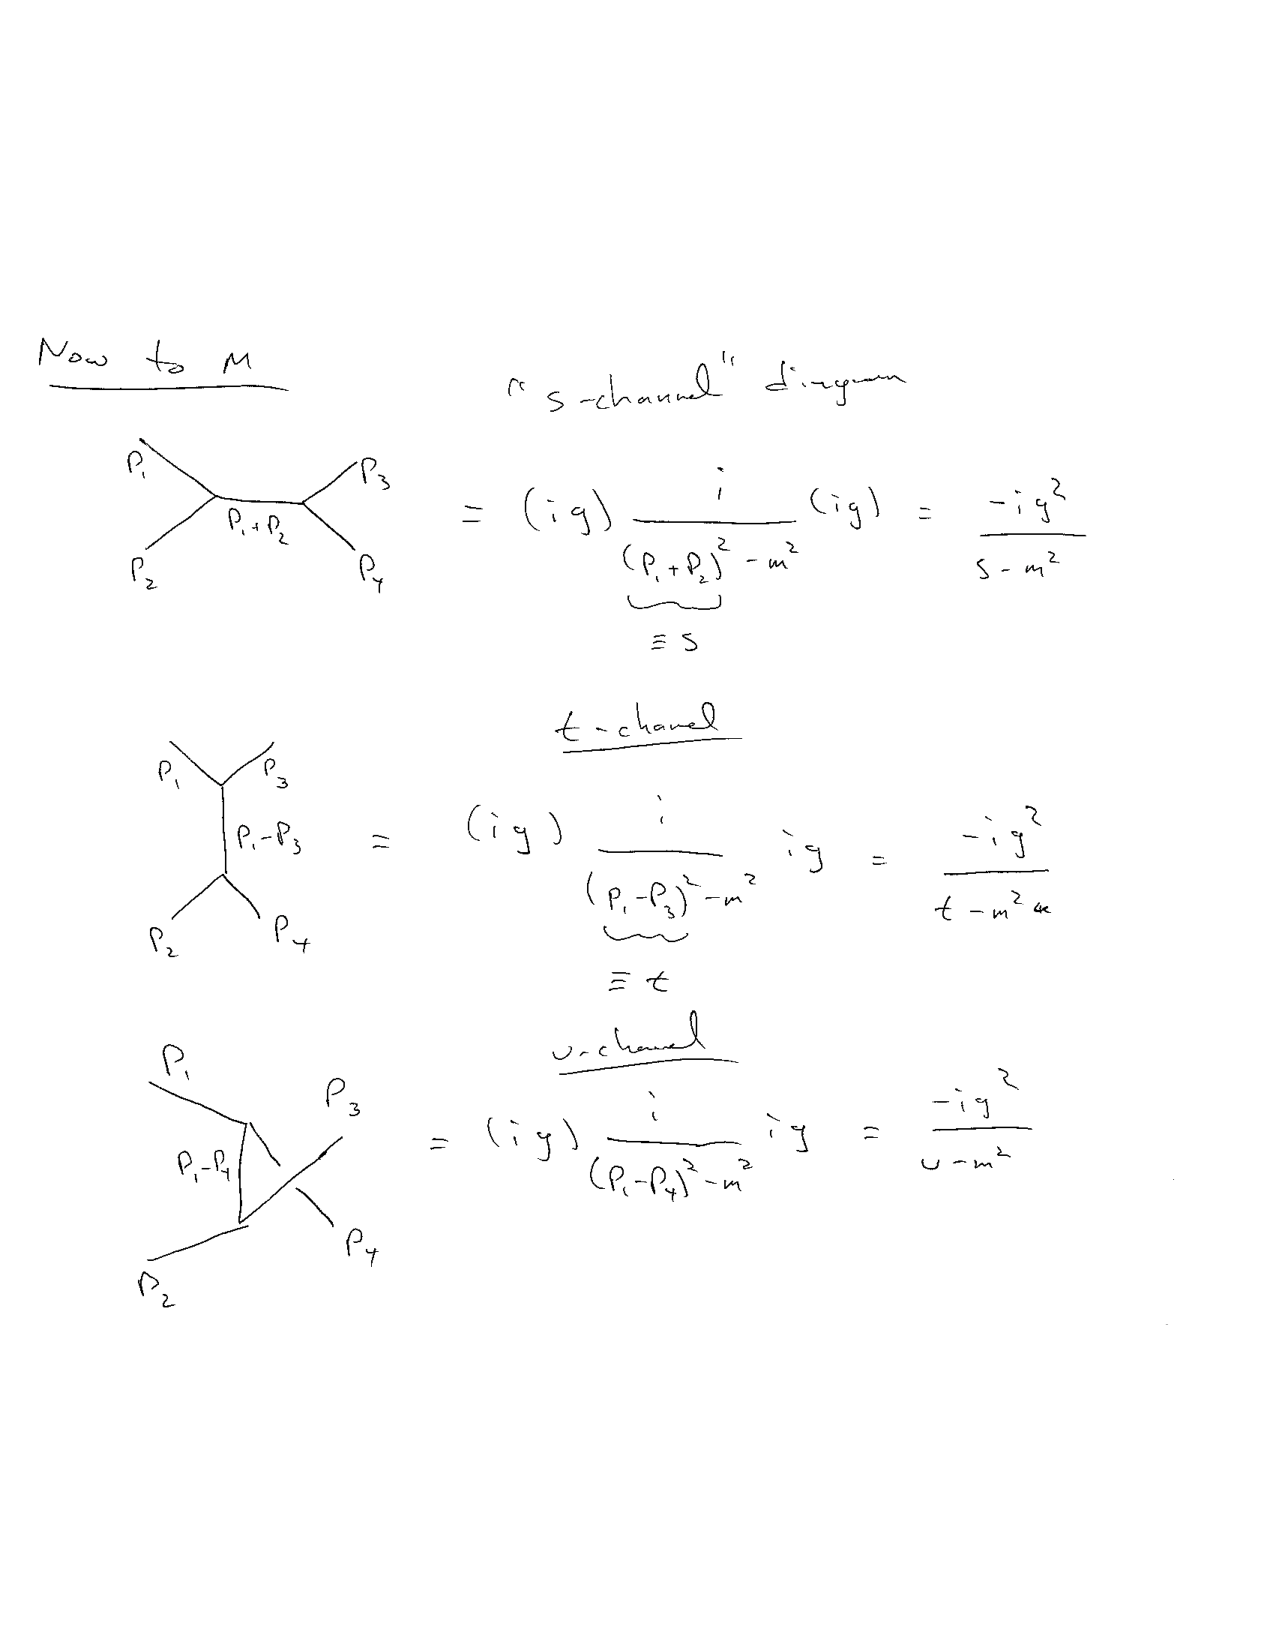
\includegraphics[width=0.99\textwidth]{./STUDiagrams.pdf}
\end{figure}

\be
\frac{d\sigma}{d\Omega}(\phi\phi\rightarrow\phi\phi) = \frac{g^4}{64 \pi^2 E_{CM}^2} \left[ \frac{1}{s-m^2} + \frac{1}{t-m^2} + \frac{1}{u-m^2} \right]
\ee


$s+t+u = \sum m_j^2$  (s,t,u are L. I)

\clearpage

\underline{Example 2} 

Electron-positron to muons scattering.

\begin{figure}[h]
\centering
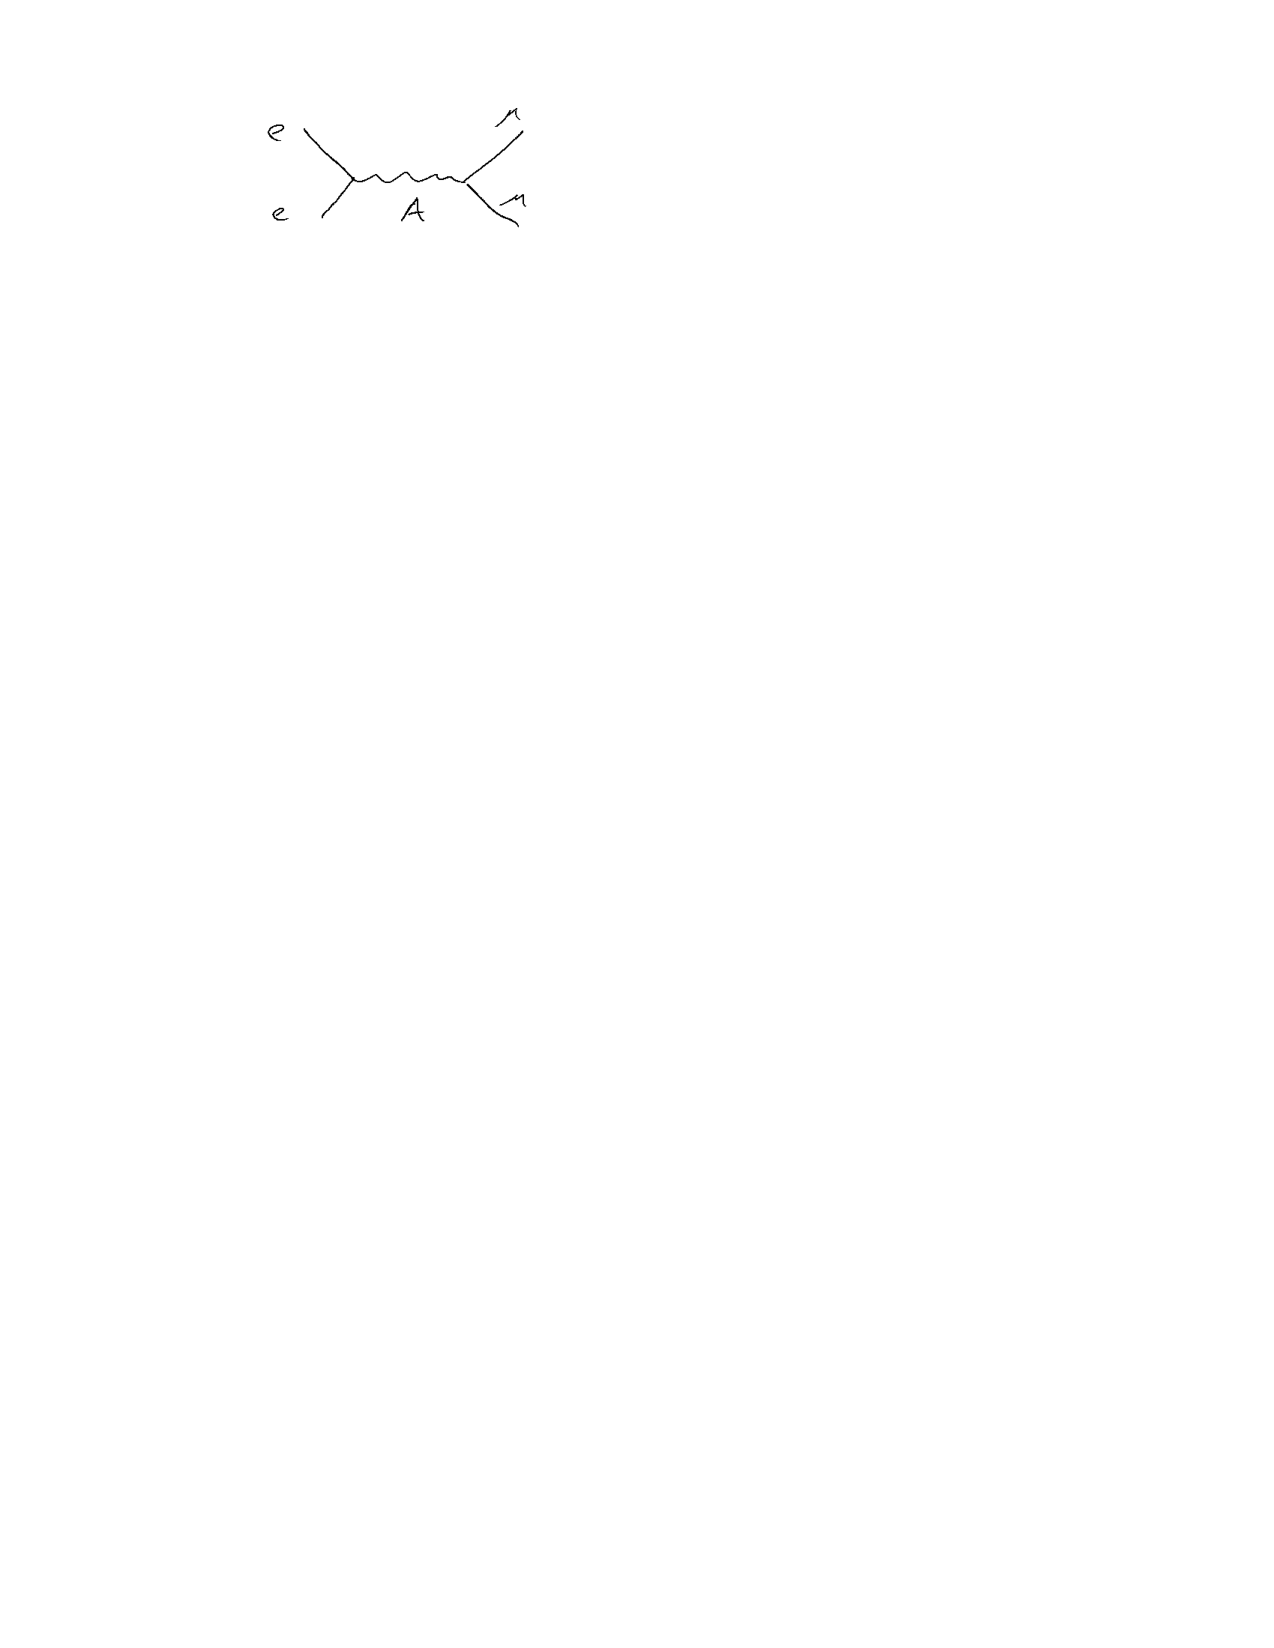
\includegraphics[width=0.5\textwidth]{./eeToMuMu.pdf}
\end{figure}

Note from:
\be
\frac{d\sigma}{d\Omega} = \frac{1}{64 \pi^2 E_{CM}^2} \frac{p_f}{p_i}  |M|^2
\ee
that M is dimensionless. 

It is given by combination of dimensionless couplings and appropriate spin projections.


Focus on the projections on
\bi
\item[-] initial spins to the $\gamma$ polarization
\item[-] $\gamma$ polarization to final spins
\ei


\be
M(s_1 s_2 \rightarrow s_3 s_4) = \underbrace{\sum_\epsilon}_{\textrm{photon polarizations}} \braket{\underbrace{s_3 s_4}_{\textrm{Spin of $\mu$s}}|\epsilon}\braket{\epsilon|\underbrace{s_1 s_2}_{\textrm{Spin of $e$s}}}
\ee

At high-energies take e and $\mu$ to be massless.


\be
P_1 = (E,0,0,E) \hspace*{1in}  P_1 = (E,0,0,-E)
\ee

In this limit think of the electron as having helicity. 


\underline{We will solve this now in linear basis} (you will do circular in HW)

\be
\ket{s_1 s_2} = \underbrace{\ket{\leftrightarrow \leftrightarrow}}_{\textrm{along-x}}, \underbrace{\ket{\updownarrow \updownarrow}}_{\textrm{along-y}}, \ket{\leftrightarrow \updownarrow}, \ket{\updownarrow \leftrightarrow}
\ee
where the spins are 1/2. 

However, only two combinations can poject onto a spin-1 photon
\be
\ket{\leftrightarrow \leftrightarrow}, \ket{\updownarrow \updownarrow}, 
\ee


\underline{photon polarizations} 

\be
\epsilon^1 = (0,1,0,0) \hspace*{1in} \epsilon^1 = (0,0,1,0)
\ee


$\ket{\leftrightarrow \leftrightarrow}$ gives $\epsilon^1$\\
$\ket{\updownarrow \updownarrow}$ gives $\epsilon^2$\\

Now, the $\mu$'s are also spin 1/2.  (Also have 4 spin states)

In general, $\mu$ not moving along same direction as the incoming electrons. 

Can paramaterize with $\theta$, (symmetric under $\phi$ can rotate such that $\phi = 0$)

\be
P_3 = E(1, 0, \sin\theta, \cos\theta ) \hspace*{1in}  P_4 = E(1, 0, -\sin\theta, -\cos\theta )
\ee

for muons, 2 possible directions of photon polarizations

\be
\bar{\epsilon}^1 = (0,1,0,0)  \hspace*{1in} \bar{\epsilon}^1 = (0,0,\cos\theta,-\sin\theta)
\ee
(Can check that these are perpindicular to $P_3$ and $P_4$)

In general,  hard to measure spins. Sum over all $\mu$ spins.

Must sum over all possible \multiline{initial \\ final} polarizations


For us only 
\bi
\item[-]$M_1 = M(\ket{\leftrightarrow \leftrightarrow} \rightarrow \ket{\bar{\epsilon^1}} = \epsilon^1 \bar{\epsilon^1} = -1$ 
\item[-]$M_2 = M(\ket{\updownarrow \updownarrow} \rightarrow \ket{\bar{\epsilon^2}} = \epsilon^2 \bar{\epsilon^2} = -cos\theta$ 
\ei
are non-zero.

If our initial beams are unpolarized, sum over initial spins. 

\be
|M|^2 = |M_1|^2 + |M_2|^2 = 1 + \cos^2\theta
\ee


\be
\frac{d\sigma}{d\Omega} \sim \frac{\alpha^2}{E_{CM}^2}(1 + \cos^2\theta)
\ee


}
\end{document}

